
\begin{figure}
\begin{subfigure}[b]{0.5\textwidth}
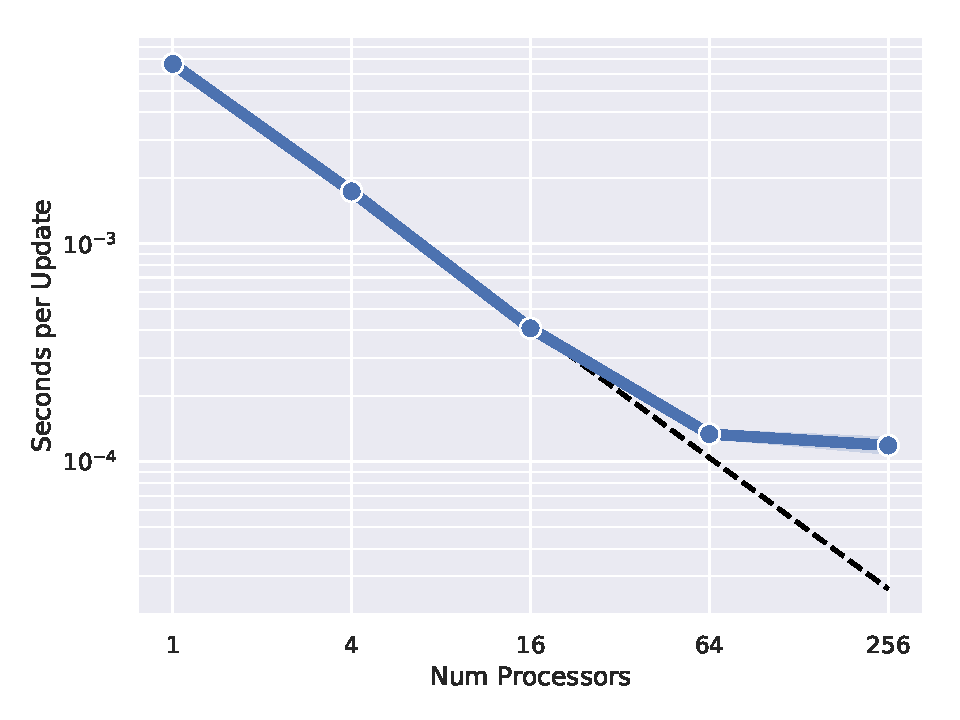
\includegraphics[width=\textwidth]{img/MPIStrong}
\caption{
MPI implementation time to solution versus parallelism for a fixed problem size (a $2048\times2048$ grid).
Dashed line indicates the ideal scaling relationship.
Shaded area represents standard deviation of five replications for each observation.
}
\label{fig:mpi_weak}
\end{subfigure}
\begin{subfigure}[b]{0.5\textwidth}
  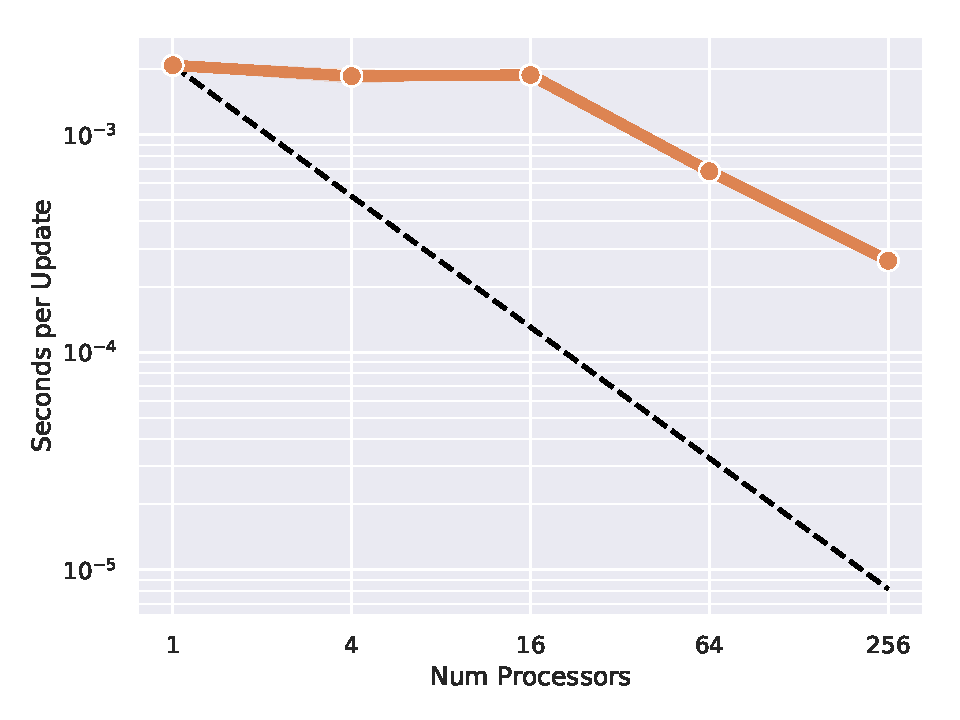
\includegraphics[width=\textwidth]{img/CharmStrong}
\caption{
Charm++ implementation time to solution versus parallelism for a fixed problem size (a $16\times16$ grid).
Dashed line denotes the ideal scaling relationship.
Shaded area represents standard deviation of five replications for each observation.
}
\label{fig:charm_weak}
\end{subfigure}
\caption{
Analogy between (\subref{fig:mpi_weak}) natural and (\subref{fig:charm_weak}) simulated hierarchical fraternal transitions of individuality.
}
\end{figure}
